\chapter{Twisted gauging and topological sectors in (2+1)d abelian lattice gauge theories}\label{app:TwistedGauging}
\section{Synopsis}
An open problem in the study of three-dimensional quantum field theories is the construction of genuinely \emph{self-dual} models --- that is, models that are mapped to themselves under some duality transformation. Necessarily, such a self-duality should preserve the symmetry structure of either model. A central observation of ref.~\cite{Decoppet2023} is that a specific class of gauging and twisted gauging transformations appears to be the only mechanism capable of producing such self-dual theories in this dimension.

The duality transformations we study in this project intertwine (2+1)-dimensional \emph{twisted Abelian lattice gauge theories} whose symmetry structure is encoded by the fusion 2-category $\TRep(G)$, which simultaneously captures Wilson line operators as 1-form symmetry operators, their condensation defects as 0-form symmetry operators, as well as topological interfaces between those membrane operators. The duality transformation amounts to the change in module 2-category $\TVect\mapsto\TVect^\alpha$ over the input $\TVect_G$, with $[\alpha]\in H^3(G,\rU(1))$ encoding the aforementioned twist or discrete torsion. Physically, this map amounts to the gauging of the 1-form symmetry of the theory, followed by a twisted gauging of the resulting 0-form $\TVect_G$ symmetry. We provide lattice representations of these symmetry operators and duality intertwiners in the form of topological matrix product operators and projected entangled-pair operators. We characterise the 1-form symmetry-twisted boundary conditions and charge sectors, and construct the unitary duality transformations that relate the dual theories to one another.

We first illustrate the mechanism in one spatial dimension, where the construction for the case of $G=\ZtZt$, with the non-trivial twist $[\psi]$ valued in $H^2(\ZtZt,\rU(1))\simeq\mbb Z_2$, reduces to the \emph{Kennedy-Tasaki duality}~\cite{Kennedy1992} and which serves as an introduction to the higher-dimensional case. In two spatial dimensions, we work out an explicit realisation of the duality between the \emph{toric code} and the \emph{double semion} model corresponding to the string-net model with $\Vect_{\mbb Z_2}$, respectively $\Vect_{\mbb Z_2}^\alpha$, as input, $[\alpha]$ being the non-trivial class in $H^3(\mbb Z_2,\rU(1))\simeq\mbb Z_2$~\cite{Kitaev1997,Levin2004,Levin2012}. Finally, we show that the sum of these two models admits an interpretation as a \emph{higher gauge theory}, in which the duality transformation is promoted to a genuine internal symmetry.
\section{Reference}
\textit{Twisted gauging and topological sectors in (2+1)d abelian lattice gauge theories} \par\noindent
\textbf{B. Vancraeynest-De Cuiper}, C. Delcamp \par\noindent
\href{https:/doi.org/10.21468/SciPostPhys.19.2.054}{SciPost Phys. \textbf{19}, 054 (2025)}, \href{https://doi.org/10.48550/arXiv.2501.16301}{arXiv:2501.16301}
\section{Contributions of the author}
This project was mainly conceived by Clement Delcamp, who developed the overarching conceptual framework based on earlier work~\cite{Delcamp2021,Delcamp2023}. He wrote the majority of the manuscript. My contributions focused primarily on the derivations related to the one-dimensional dualities, including the mapping of topological sectors and order parameters. I additionally contributed to the two-dimensional case, in particular with regard to the symmetries and boundary conditions of the two-dimensional models. I also co-wrote sections of the paper.
%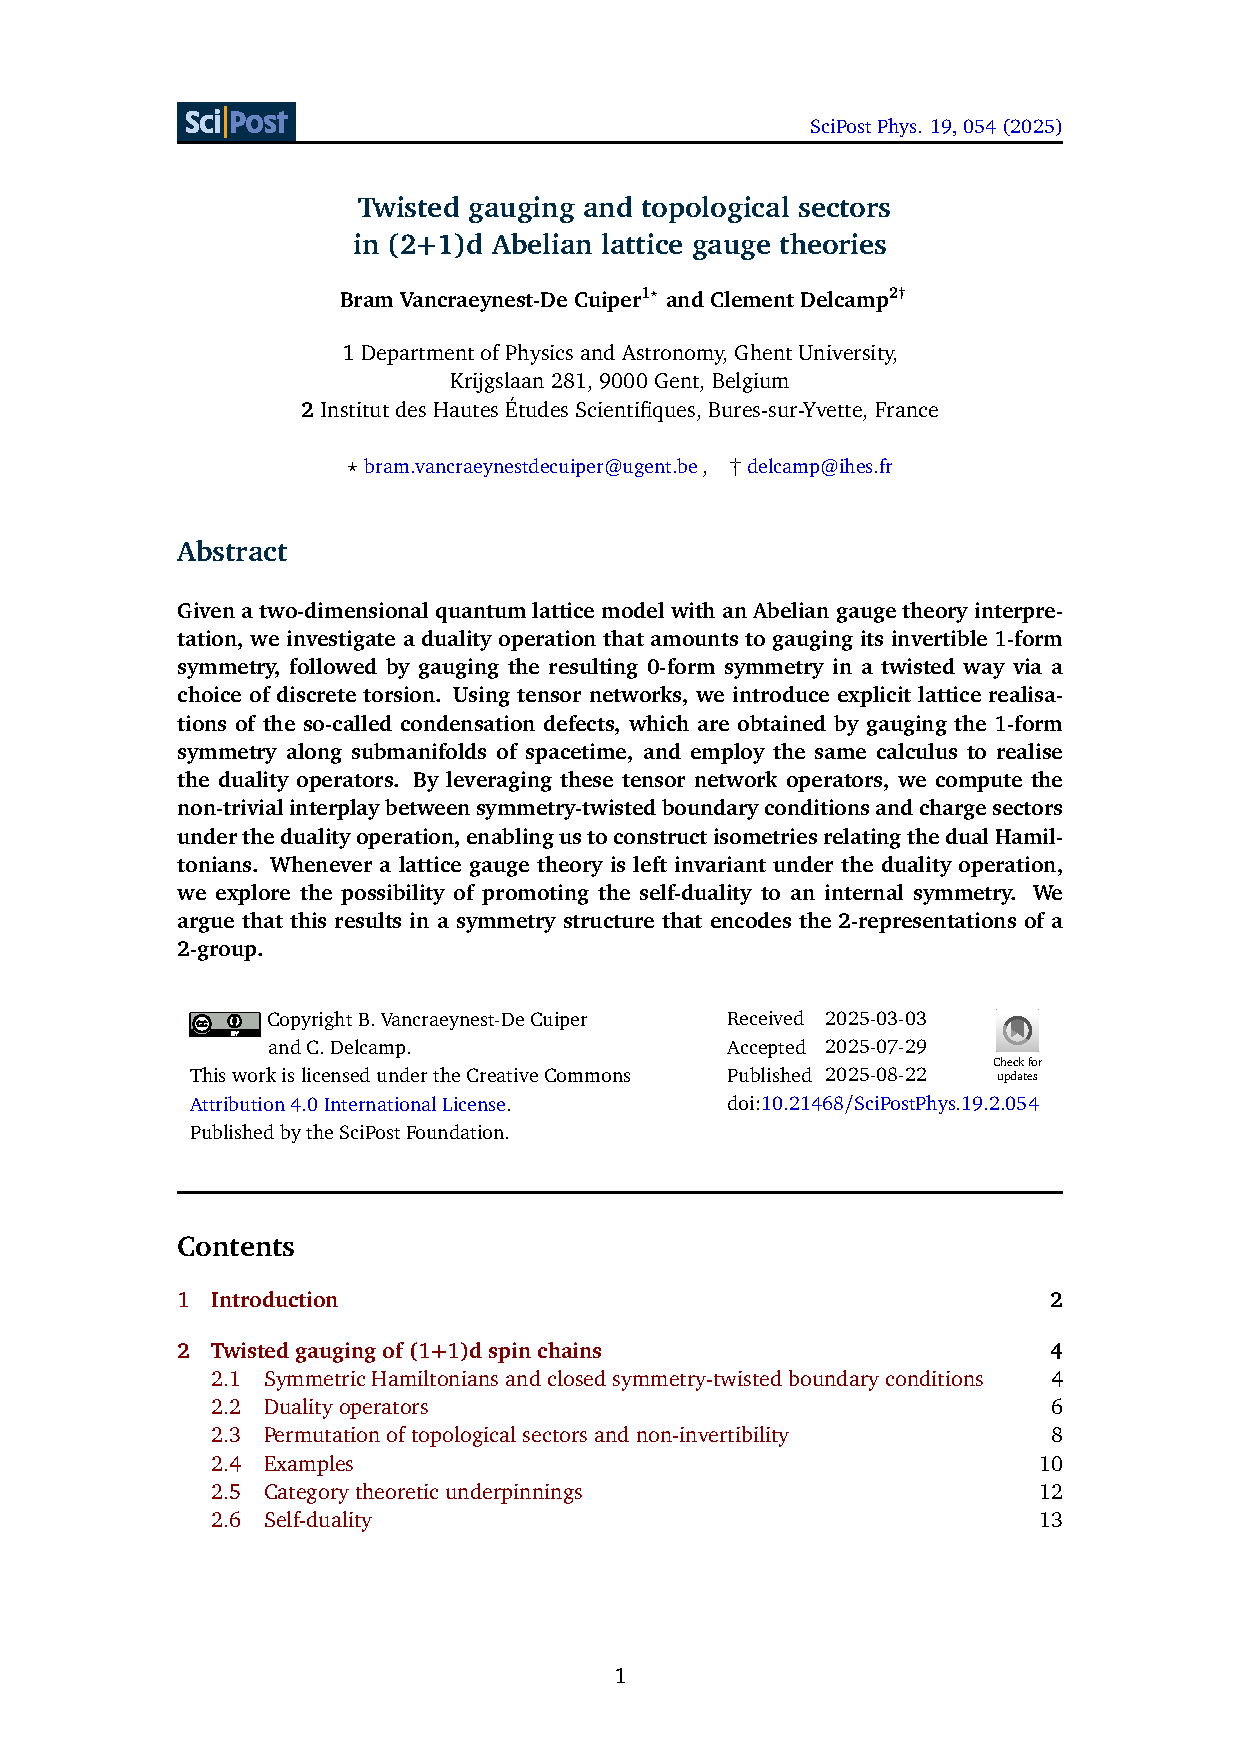
\includepdf[pages=-, trim=1.3cm 1.8cm 1.3cm 0cm, offset=-4mm 7mm, clip=true, frame=false, noautoscale=true, width=1.08\headwidth, pagecommand={}]{papers/twisted_gauging}
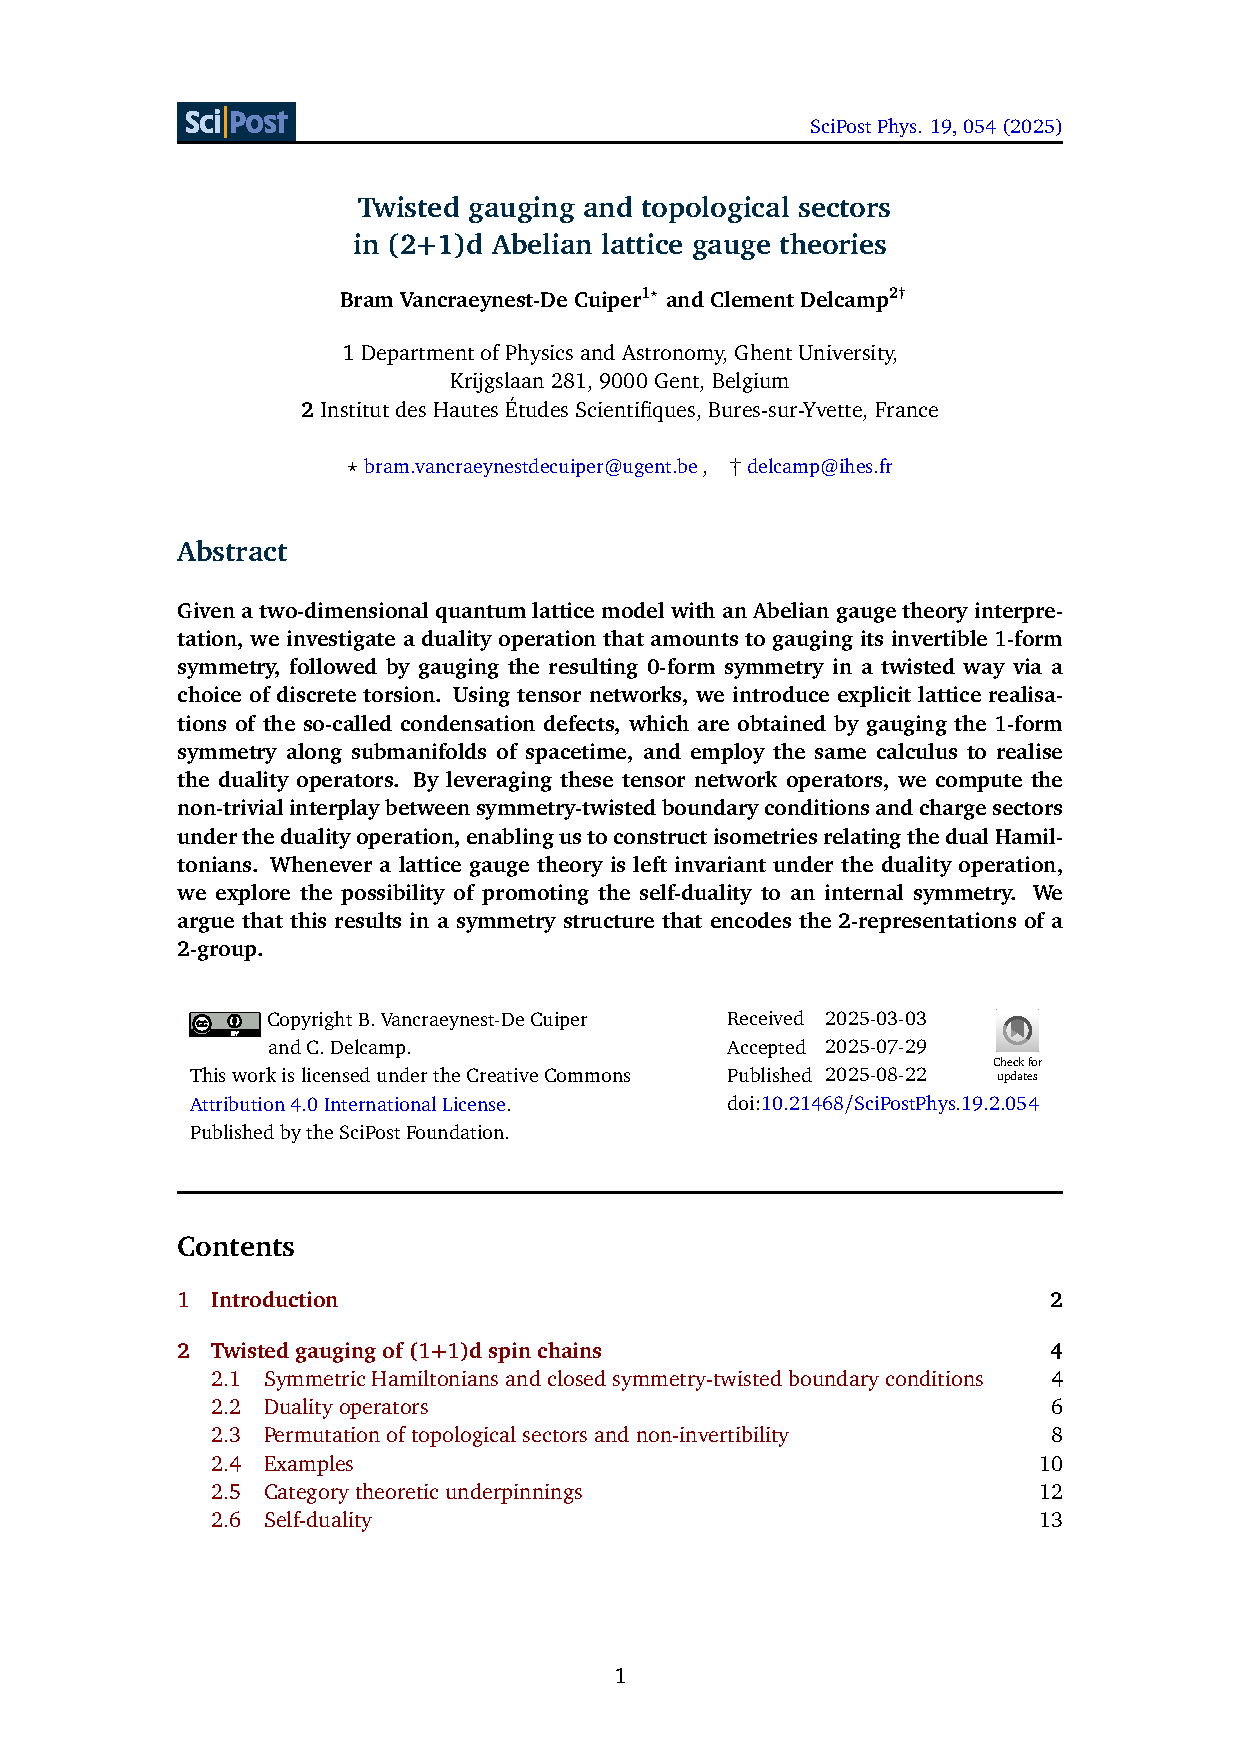
\includepdf[pages=-,
trim=25mm 20.54mm 25mm 17mm, clip=true,
noautoscale=true, height=\textheight,
offset=-0.65mm 4mm,
pagecommand={\thispagestyle{publication}}]{papers/twisted_gauging}